\documentclass[conference,a4paper,10pt, oneside,final]{tfmpd}
%\usepackage[latin1]{inputenc}   % caracteres especiales (acentos, eñes)
%\usepackage[spanish]{babel}     % varias definiciones para el español
\usepackage[utf8x]{inputenc}
\usepackage{graphicx}           % inserción de graficos
\usepackage{float} %paquete para que ponga las imagenees donde yo quiero, no donde quiere el muy hdp de latex
%la posición de la imagen, con H (mayúscula!!)

\usepackage{amssymb}
\usepackage{amsfonts}
\usepackage{amsmath}

\begin{document}

\title{Técnicas de Eseganografía en señales de audio.}

\author{Darío A. Villarreal,
        Esteban J. Zeller y
        Matías A. Eberhardt\\
\textit{Trabajo Práctico Final de Procesamiento Digital de Señales, II-FICH-UNL.}}

\markboth{Trabajo Práctico Final de Procesamiento Digital de Señales}{}

\maketitle

\begin{abstract}
En este trabajo haremos una breve clasificación de las técnicas de esteganografía existentes y su diferenciación con otras disciplinas de protección de datos digitales. Luego decribiremos e implementaremos dos de dichas técnicas: Modificación del Bit Menos Significativo (LSB, Least Significant Bit) en el dominio temporal y en el dominio frecuencial se ocultará la información en los coeficientes de la Tranformada Wavelet Discreta. Finalmente evaluaremos los resultados obtenidos mediante técnicas objetivas y subjetivas.
\end{abstract}

\begin{keywords}
esteganografía, data hidding, watermarking
\end{keywords}

\section{Introducción}
\PARstart{L}{a} esteganografía es una disciplina que se dedica a ocultar mensajes u objetos dentro de otros llamados portadores de modo que su inclusión pase desapercibida. Básicamente explota las limitaciones de la percepción humana, ya que nuestros sentidos presentan límites para percibir pequeñas alteraciones en las señales.
Pese a que es usada desde la antigüedad, esta disciplina ha suscitado mucho interés en las últimas décadas, especialmente en el área de la seguridad de la información dado el crecimiento del uso de la red de comunicaciones. La gran cantidad de información digital que circula en ella ha hecho que profesionales de la industria e investigadores prestaran especial atención en la seguridad de los datos digitales, siendo las principales disciplinas la criptografía, esteganografía y watermarking. 

\begin{figure}[h!]
 \centering
 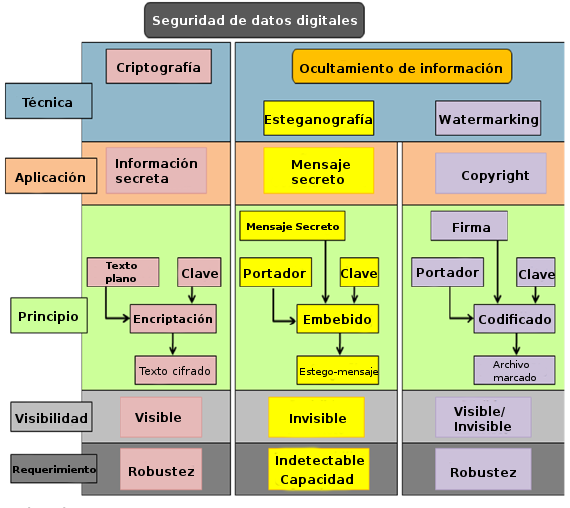
\includegraphics[keepaspectratio=true, width=250 px]{./cuadro.png}
 % cuadro.png: 0x0 pixel, 300dpi, 0.00x0.00 cm, bb=
 \caption{Disciplinas de segudidad de datos digitales}
 \label{fig: Disciplinas de segudidad de datos digitales}
\end{figure}

La criptografía busca evitar que cierta información pueda ser leída por personas sin autorización, por lo que su principal requerimiento es la robustez ante los intentos de descifrado. El watermarking busca dejar una huella (visible o invisible) identificable y robusta ante ataques y compresión en imágenes, audio y vídeo. Para el diseño de técnicas esteganográficas los tres parámetros a tener en cuenta son la capacidad de ocultamiento de información, la imperceptibilidad y la robustez, pero es imposible obtenerlos al mismo tiempo. Por ejemplo, los métodos con más capacidad son sensibles al ruido y la compresión, mientras que los métodos robustos presentan una baja capacidad de ocultamiento de información.

Entre las aplicaciones prácticas de la esteganografía digital se encuentran la conunicación encubierta, inclusión de copyright en archivos multimedia, ocultar ejecutables para obtener datos de uso o acceso a un equipo remoto, entre otros.

En este trabajo repasaremos brevemente las principales técnicas de esteganografía digital en archivos de audio, luego implementaremos dos de ellas y finalmente analizaremos los resultados obtenidos.

\section{Clasificación de métodos esteganográficos}

\subsection{En el dominio del tiempo}
\subsubsection{Bit menos significativo} Se trata de embeber la información modificando los bits menos significativos de una señal. Presenta imperceptibilidad con una alta capacidad de ocultamiento de información. Dado que es el método mas simple, la seguridad del canal de información se ve fácilmente comprometida bajo un simple análisis de los bits menos significativos. Para evitar que la información pueda ser reconstruida por personas sin autorización, se pueden tomar las siguientes medidas: encriptar el mensaje antes de su embebido, seleccionar el bit a codificar y el siguiente frame que contandrá información mediante los bits mas significativos del frame.
El método es muy suceptible a ruidos, compresión y filtrado, los cuales eliminan o deterioran el mensaje oculto.

\subsubsection{Echo hidding}
Esta técnica se basa en introducir pequeños ecos en la señal portadora, mediante la convolución en el tiempo con
un impulso determinado, quedando la señal con las mismas características estadísticas y perceptivas. La información es ocultada manipulando tres parámetros de la señal de eco: la amplitud inicial, el offset y la tasa de decaimiento. Esta técnica prácticamente no es utilizada debido a su baja capacidad de embebido y robustez.

\subsubsection{Intérvalos de silencio}
Este método consiste en embeber la información en los intervalos de silencio en una señal de habla. Primero se determina la cantidad y duración de dichos intervalos en muestras para luego disminuir su duración restándole x cantidad de muestras, donde $0 < x < 2^{nbits}$ y $nbits$ es la cantidad de bits necesarios para representar un valor del mensaje a ocultar. En el proceso de extracción, se calcula el módulo entre la longitud del intervalo y nbits para recuperar el valor oculto. Este metodo presenta una alta imperceptibilidad, pero baja capacidad. Presenta robustez antes ruido y filtrado, pero no ante algunos algoritmos de compresión.


\subsection{En el dominio de la frecuencia}
\subsubsection{Magnitud del espectro}
\subsubsection{Inserción de tono}
\subsubsection{Espectro de fase}
\subsubsection{Amplio espectro}
\subsubsection{Dominio Cepstral}
\subsubsection{Wavelets}

\subsection{En la codificación/decodificación}
\subsubsection{Modicicación de los codebooks}
\subsubsection{Ocultamiento en el fujo de bits}

\section{Implementación en el dominio temporal}
\section{Implementación en el dominio frecuencial}
\section{Evaluación de resultados}
\section{Conclusiones}

\nocite{*}
\bibliographystyle{tfmpd}
\bibliography{tfmpd}

\end{document}
